\documentclass[border=5px]{standalone}
\usepackage{tikz}
\usetikzlibrary{shapes}
\begin{document}
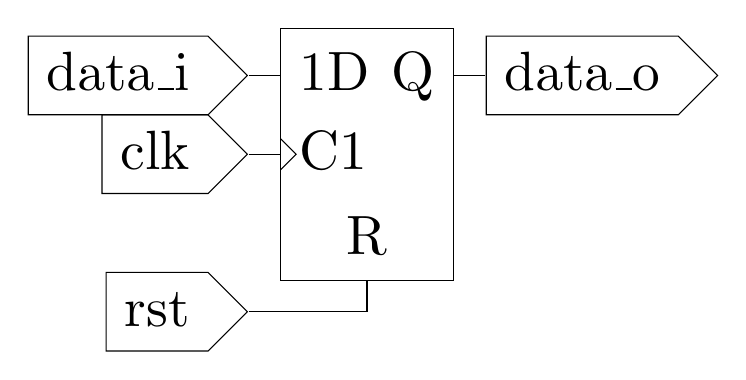
\begin{tikzpicture}[text height=1.5ex,text depth=.25ex,scale=2,transform shape]
  \draw (0.2,0.2) rectangle (1.3,1.8);
  \draw (0,1.5) node[signal,signal to=east,draw,anchor=east] {data\_i} -- (0.2,1.5) node[anchor=west]{1D};
  \draw (0,1.0) node[signal,signal to=east,draw,anchor=east] {clk} -- (0.2,1.0) node[anchor=west] {C1};
  \draw (0,0) node[signal,signal to=east,draw,anchor=east] {rst} -| (0.75,0.2) node[anchor=south]{R};
  \draw (0.2,1.1) -- (0.3,1.0) -- (0.2,0.9);
  \draw (1.5,1.5) node[signal,signal to=east,draw,anchor=west] {data\_o} -- (1.3,1.5) node[anchor=east] {Q};
\end{tikzpicture}
\end{document}
